%% uncomment to list all files in log
%\listfiles

\documentclass[12pt]{report}


\usepackage{fontspec}

%\setmainfont[Scale=MatchLowercase]{Lucida Bright}
%\setmonofont{FreeMono}
%\setmonofont{Source Code Pro}
\setmonofont[Scale=MatchLowercase]{Ubuntu Mono}

\usepackage[headings]{fullpage}

% national use characters 
%\usepackage{inputenc}

% ams mathematical symbols
\usepackage{amsmath,amssymb}

% added to support pandoc highlighting
\usepackage{microtype}

\usepackage{makeidx}

% add index and bibliographies to table of contents
\usepackage[nottoc]{tocbibind}

% postscript courier and times in place of cm fonts
%\usepackage{courier}
%\usepackage{times}

% extended coloring
\usepackage{color}
\usepackage[table,dvipsnames]{xcolor}
\usepackage{colortbl}

% advanced date formating
\usepackage{datetime}

%support pandoc code highlighting
\usepackage{fancyvrb}
\DefineShortVerb[commandchars=\\\{\}]{\|}
\DefineVerbatimEnvironment{Highlighting}{Verbatim}{commandchars=\\\{\}}
% Add ',fontsize=\small' for more characters per line

%tango style colors
% \usepackage{framed}
% \definecolor{shadecolor}{RGB}{255,255,255}
% \newenvironment{Shaded}{\begin{snugshade}}{\end{snugshade}}
% \newcommand{\KeywordTok}[1]{\textcolor[rgb]{0.13,0.29,0.53}{\textbf{{#1}}}}
% \newcommand{\DataTypeTok}[1]{\textcolor[rgb]{0.13,0.29,0.53}{{#1}}}
% \newcommand{\DecValTok}[1]{\textcolor[rgb]{0.00,0.00,0.81}{{#1}}}
% \newcommand{\BaseNTok}[1]{\textcolor[rgb]{0.00,0.00,0.81}{{#1}}}
% \newcommand{\FloatTok}[1]{\textcolor[rgb]{0.00,0.00,0.81}{{#1}}}
% \newcommand{\CharTok}[1]{\textcolor[rgb]{0.31,0.60,0.02}{{#1}}}
% \newcommand{\StringTok}[1]{\textcolor[rgb]{0.31,0.60,0.02}{{#1}}}
% \newcommand{\CommentTok}[1]{\textcolor[rgb]{0.56,0.35,0.01}{\textit{{#1}}}}
% \newcommand{\OtherTok}[1]{\textcolor[rgb]{0.56,0.35,0.01}{{#1}}}
% \newcommand{\AlertTok}[1]{\textcolor[rgb]{0.94,0.16,0.16}{{#1}}}
% \newcommand{\FunctionTok}[1]{\textcolor[rgb]{0.00,0.00,0.00}{{#1}}}
% \newcommand{\RegionMarkerTok}[1]{{#1}}
% \newcommand{\ErrorTok}[1]{\textbf{{#1}}}
% \newcommand{\NormalTok}[1]{{#1}}

%espresso style colors
% \usepackage{framed}
% \definecolor{shadecolor}{RGB}{42,33,28}
% \newenvironment{Shaded}{\begin{snugshade}}{\end{snugshade}}
% \newcommand{\KeywordTok}[1]{\textcolor[rgb]{0.26,0.66,0.93}{\textbf{{#1}}}}
% \newcommand{\DataTypeTok}[1]{\textcolor[rgb]{0.74,0.68,0.62}{\underline{{#1}}}}
% \newcommand{\DecValTok}[1]{\textcolor[rgb]{0.27,0.67,0.26}{{#1}}}
% \newcommand{\BaseNTok}[1]{\textcolor[rgb]{0.27,0.67,0.26}{{#1}}}
% \newcommand{\FloatTok}[1]{\textcolor[rgb]{0.27,0.67,0.26}{{#1}}}
% \newcommand{\CharTok}[1]{\textcolor[rgb]{0.02,0.61,0.04}{{#1}}}
% \newcommand{\StringTok}[1]{\textcolor[rgb]{0.02,0.61,0.04}{{#1}}}
% \newcommand{\CommentTok}[1]{\textcolor[rgb]{0.00,0.40,1.00}{\textit{{#1}}}}
% \newcommand{\OtherTok}[1]{\textcolor[rgb]{0.74,0.68,0.62}{{#1}}}
% \newcommand{\AlertTok}[1]{\textcolor[rgb]{1.00,1.00,0.00}{{#1}}}
% \newcommand{\FunctionTok}[1]{\textcolor[rgb]{1.00,0.58,0.35}{\textbf{{#1}}}}
% \newcommand{\RegionMarkerTok}[1]{\textcolor[rgb]{0.74,0.68,0.62}{{#1}}}
% \newcommand{\ErrorTok}[1]{\textcolor[rgb]{0.74,0.68,0.62}{\textbf{{#1}}}}
% \newcommand{\NormalTok}[1]{\textcolor[rgb]{0.74,0.68,0.62}{{#1}}}

%kete style colors
% \newenvironment{Shaded}{}{}
% \newcommand{\KeywordTok}[1]{\textbf{{#1}}}
% \newcommand{\DataTypeTok}[1]{\textcolor[rgb]{0.50,0.00,0.00}{{#1}}}
% \newcommand{\DecValTok}[1]{\textcolor[rgb]{0.00,0.00,1.00}{{#1}}}
% \newcommand{\BaseNTok}[1]{\textcolor[rgb]{0.00,0.00,1.00}{{#1}}}
% \newcommand{\FloatTok}[1]{\textcolor[rgb]{0.50,0.00,0.50}{{#1}}}
% \newcommand{\CharTok}[1]{\textcolor[rgb]{1.00,0.00,1.00}{{#1}}}
% \newcommand{\StringTok}[1]{\textcolor[rgb]{0.87,0.00,0.00}{{#1}}}
% \newcommand{\CommentTok}[1]{\textcolor[rgb]{0.50,0.50,0.50}{\textit{{#1}}}}
% \newcommand{\OtherTok}[1]{{#1}}
% \newcommand{\AlertTok}[1]{\textcolor[rgb]{0.00,1.00,0.00}{\textbf{{#1}}}}
% \newcommand{\FunctionTok}[1]{\textcolor[rgb]{0.00,0.00,0.50}{{#1}}}
% \newcommand{\RegionMarkerTok}[1]{{#1}}
% \newcommand{\ErrorTok}[1]{\textcolor[rgb]{1.00,0.00,0.00}{\textbf{{#1}}}}
% \newcommand{\NormalTok}[1]{{#1}}
%end pandoc code hacks

% jodliterate colors
\usepackage{color}
\definecolor{shadecolor}{RGB}{248,248,248}
% j control structures 
\definecolor{keywcolor}{rgb}{0.13,0.29,0.53}
% j explicit arguments x y m n u v
\definecolor{datacolor}{rgb}{0.13,0.29,0.53}
% j numbers - all types see j.xml
\definecolor{decvcolor}{rgb}{0.00,0.00,0.81}
\definecolor{basencolor}{rgb}{0.00,0.00,0.81}
\definecolor{floatcolor}{rgb}{0.00,0.00,0.81}
% j local assignments
\definecolor{charcolor}{rgb}{0.31,0.60,0.02}
\definecolor{stringcolor}{rgb}{0.31,0.60,0.02}
\definecolor{commentcolor}{rgb}{0.56,0.35,0.01}
% primitive adverbs and conjunctions
%\definecolor{othercolor}{rgb}{0.56,0.35,0.01}   
\definecolor{othercolor}{RGB}{0,0,255}
% global assignments
\definecolor{alertcolor}{rgb}{0.94,0.16,0.16}
% primitive J verbs and noun names
\definecolor{funccolor}{rgb}{0.00,0.00,0.00}    

\usepackage{framed}
\newenvironment{Shaded}{}{}
\newcommand{\KeywordTok}[1]{\textcolor{keywcolor}{\textbf{{#1}}}}
\newcommand{\DataTypeTok}[1]{\textcolor{datacolor}{{#1}}}
%\newcommand{\DecValTok}[1]{\textcolor{decvcolor}{{#1}}}
\newcommand{\DecValTok}[1]{{#1}} 
\newcommand{\BaseNTok}[1]{\textcolor{basencolor}{{#1}}}
\newcommand{\FloatTok}[1]{\textcolor{floatcolor}{{#1}}}
\newcommand{\CharTok}[1]{\textcolor{charcolor}{\textbf{{#1}}}}
\newcommand{\StringTok}[1]{\textcolor{stringcolor}{{#1}}}
\newcommand{\CommentTok}[1]{\textcolor{commentcolor}{\textit{{#1}}}}
\newcommand{\OtherTok}[1]{\textcolor{othercolor}{{#1}}} 
\newcommand{\AlertTok}[1]{\textcolor{alertcolor}{\textbf{{#1}}}}
%\newcommand{\FunctionTok}[1]{\textcolor{funccolor}{{#1}}}
\newcommand{\FunctionTok}[1]{{#1}}
\newcommand{\RegionMarkerTok}[1]{{#1}}
\newcommand{\ErrorTok}[1]{\textbf{{#1}}}
\newcommand{\NormalTok}[1]{{#1}}

% headers and footers
\usepackage{fancyhdr}
\pagestyle{fancy}

\fancyhead{}
\fancyfoot{}

%\fancyhead[LE,RO]{\slshape \rightmark}
%\fancyhead[LO,RE]{\slshape \leftmark}
\fancyfoot[C]{\thepage}
%\headrulewidth 0.4pt
%\footrulewidth 0 pt

%\addtolength{\headheight}{\baselineskip}

%\lfoot{\emph{Analyze the Data not the Drivel}}
%\rfoot{\emph{\today}}

% subfigure handles figures that contain subfigures
%\usepackage{color,graphicx,subfigure,sidecap}
\usepackage{graphicx,sidecap}
\usepackage{subfigure}
\graphicspath{{./inclusions/}}

% floatflt provides for text wrapping around small figures and tables
\usepackage{floatflt}

% tweak caption formats 
\usepackage{caption} 
\usepackage{sidecap}
%\usepackage{subcaption} % not compatible with subfigure

\usepackage{rotating} % flip tables sideways

% complex footnotes
%\usepackage{bigfoot}

% weird logos \XeLaTeX
\usepackage{metalogo}

% source code listings
\usepackage{listings}

% long tables
% \usepackage{longtable}

\newcommand{\HRule}{\rule{\linewidth}{0.5mm}}

% map LaTeX cross references into PDF cross references
\usepackage[
            %dvips,
            colorlinks,
            linkcolor=blue,
            citecolor=blue,
            urlcolor=blue,   % magenta, cyan default        
            pdfauthor={John D. Baker},
            pdftitle={Analyze the Data not the Drivel},
            pdfsubject={Blog},
            pdfcreator={MikTeX+LaTeXe with hyperref package},
            pdfkeywords={blog,wordpress},
            ]{hyperref}
           
% custom colors
\definecolor{CodeBackGround}{cmyk}{0.0,0.0,0,0.05}    % light gray
\definecolor{CodeComment}{rgb}{0,0.50,0.00}           % dark green {0,0.45,0.08}
\definecolor{TableStripes}{gray}{0.9}                 % odd/even background in tables

\lstdefinelanguage{bat}
{morekeywords={echo,title,pushd,popd,setlocal,endlocal,off,if,not,exist,set,goto,pause},
sensitive=True,
morecomment=[l]{rem}
}

\lstdefinelanguage{jdoc}
{
morekeywords={},
otherkeywords={assert.,break.,continue.,for.,do.,if.,else.,elseif.,return.,select.,end.
,while.,whilst.,throw.,catch.,catchd.,catcht.,try.,case.,fcase.},
sensitive=True,
morecomment=[l]{NB.},
morestring=[b]',
morestring=[d]',
}

% latex size ordering - can never remember it
% \tiny
% \scriptsize
% \footnotesize
% \small
% \normalsize
% \large
% \Large
% \LARGE
% \huge
% \Huge
 
% listings package settings  
\lstset{%
  language=jdoc,                                % j document settings
  basicstyle=\ttfamily\footnotesize,            
  keywordstyle=\bfseries\color{keywcolor}\footnotesize,
  identifierstyle=\color{black},
  commentstyle=\slshape\color{CodeComment},     % colored slanted comments
  stringstyle=\color{red}\ttfamily,
  showstringspaces=false,                       
  %backgroundcolor=\color{CodeBackGround},       
  frame=single,                                
  framesep=1pt,                                 
  framerule=0.8pt,                             
  rulecolor=\color{CodeBackGround},   
  showspaces=false,
  %columns=fullflexible,
  %numbers=left,
  %numberstyle=\footnotesize,
  %numbersep=9pt,
  tabsize=2,
  showtabs=false,
  captionpos=b
  breaklines=true,                              
  breakindent=5pt                              
}

\lstdefinelanguage{JavaScript}{
  keywords={typeof, new, true, false, catch, function, return, null, catch, switch, var, if, in, while, do, else, case, break},
  ndkeywords={class, export, boolean, throw, implements, import, this},
  ndkeywordstyle=\color{darkgray}\bfseries,
  sensitive=false,
  comment=[l]{//},
  morecomment=[s]{/*}{*/},
  morestring=[b]',
  morestring=[b]"
}

% C# settings
\lstdefinestyle{sharpc}{
language=[Sharp]C,
basicstyle=\ttfamily\scriptsize, 
keywordstyle=\bfseries\color{keywcolor}\scriptsize,
framerule=0pt
}

% for source code listing longer than two use smaller font
\lstdefinestyle{smallersource}{
basicstyle=\ttfamily\scriptsize, 
keywordstyle=\bfseries\color{keywcolor}\scriptsize,
framerule=0pt
}

\lstdefinestyle{resetdefaults}{
language=jdoc,
basicstyle=\ttfamily\footnotesize,  
keywordstyle=\bfseries\color{keywcolor}\footnotesize,                                                               
framerule=0.8pt 
}

% APL UTF8 code points listed for lstlisting processing
\makeatletter
\lst@InputCatcodes
\def\lst@DefEC{%
 \lst@CCECUse \lst@ProcessLetter
  ^^80^^81^^82^^83^^84^^85^^86^^87^^88^^89^^8a^^8b^^8c^^8d^^8e^^8f%
  ^^90^^91^^92^^93^^94^^95^^96^^97^^98^^99^^9a^^9b^^9c^^9d^^9e^^9f%
  ^^a0^^a1^^a2^^a3^^a4^^a5^^a6^^a7^^a8^^a9^^aa^^ab^^ac^^ad^^ae^^af%
  ^^b0^^b1^^b2^^b3^^b4^^b5^^b6^^b7^^b8^^b9^^ba^^bb^^bc^^bd^^be^^bf%
  ^^c0^^c1^^c2^^c3^^c4^^c5^^c6^^c7^^c8^^c9^^ca^^cb^^cc^^cd^^ce^^cf%
  ^^d0^^d1^^d2^^d3^^d4^^d5^^d6^^d7^^d8^^d9^^da^^db^^dc^^dd^^de^^df%
  ^^e0^^e1^^e2^^e3^^e4^^e5^^e6^^e7^^e8^^e9^^ea^^eb^^ec^^ed^^ee^^ef%
  ^^f0^^f1^^f2^^f3^^f4^^f5^^f6^^f7^^f8^^f9^^fa^^fb^^fc^^fd^^fe^^ff%
  ^^^^20ac^^^^0153^^^^0152%
  ^^^^20a7^^^^2190^^^^2191^^^^2192^^^^2193^^^^2206^^^^2207^^^^220a%
  ^^^^2218^^^^2228^^^^2229^^^^222a^^^^2235^^^^223c^^^^2260^^^^2261%
  ^^^^2262^^^^2264^^^^2265^^^^2282^^^^2283^^^^2296^^^^22a2^^^^22a3%
  ^^^^22a4^^^^22a5^^^^22c4^^^^2308^^^^230a^^^^2336^^^^2337^^^^2339%
  ^^^^233b^^^^233d^^^^233f^^^^2340^^^^2342^^^^2347^^^^2348^^^^2349%
  ^^^^234b^^^^234e^^^^2350^^^^2352^^^^2355^^^^2357^^^^2359^^^^235d%
  ^^^^235e^^^^235f^^^^2361^^^^2362^^^^2363^^^^2364^^^^2365^^^^2368%
  ^^^^236a^^^^236b^^^^236c^^^^2371^^^^2372^^^^2373^^^^2374^^^^2375%
  ^^^^2377^^^^2378^^^^237a^^^^2395^^^^25af^^^^25ca^^^^25cb%  
  ^^00}
\lst@RestoreCatcodes
\makeatother

% custom lengths used within minipages
\newcommand{\minindent}{17pt}


\makeindex

\begin{document}

\subsection*{\href{https://bakerjd99.wordpress.com/2012/02/25/wordpress-to-LaTeX-with-pandoc-and-j-using-texfrwpxml-ijs-part-3/}{WordPress to \LaTeX\ with Pandoc and J: Using \texttt{TeXfrWpxml.ijs} (3)}}
\addcontentsline{toc}{subsection}{WordPress to \LaTeX\ with Pandoc and J: Using \texttt{TeXfrWpxml.ijs} (Part 3)}


\noindent\emph{Posted: 26 Feb 2012 02:38:53}
\vspace{6pt}

%{[}caption id=``'' align=``alignright'' width=``150''  caption=``WordPress to  LaTeX''{]}
%
\includegraphics{i-mNK4RHL-M.png}
%{[}/caption{]}
\captionsetup[floatingfigure]{labelformat=empty}
\begin{floatingfigure}[r]{0.23\textwidth}
\centering

\includegraphics[width=0.22\textwidth]{i-mNK4RHL-M.png}
\caption{WordPress to  \LaTeX}
\label{fig:2518X0}
\end{floatingfigure}In this post I will describe how to use the J script
\href{http://www.box.com/s/9v5b6ub9cya108c03mr7}{\texttt{TeXfrWpxml.ijs}}
to generate \LaTeX\ source from WordPress export XML. I am assuming you
have worked through
\href{http://bakerjd99.wordpress.com/2012/02/11/wordpress-to-latex-with-pandoc-and-j-prerequisites-part-1/}{(Part
1)} and
\href{http://bakerjd99.wordpress.com/2012/02/18/wordpress-to-latex-with-pandoc-and-j-latex-directories-part-2-2/}{(Part
2)} and have:

\begin{enumerate}
\item
  Successfully installed and tested
  \href{http://johnmacfarlane.net/pandoc/}{Pandoc}.
\item
  Installed and tested \href{http://www.jsoftware.com/}{a version of J}.
\item
  Set up appropriate directories
  (\href{http://bakerjd99.wordpress.com/2012/02/18/wordpress-to-latex-with-pandoc-and-j-latex-directories-part-2-2/}{Part
  2}).
\item
  Know how to use \LaTeX.
\end{enumerate}
Item \#4 is a \emph{big} if. Inexperienced \LaTeX\ users will probably not
enjoy a lot of success with this procedure as the source generated by
\texttt{TeXfrWpxml.ijs} requires manual edits to produce good results.
However, if you're not a \LaTeX\ guru, do not get discouraged. It's not
difficult to create blog documents like
\href{http://www.box.com/s/8yvm27ag9agtm32nfahd}{\texttt{bm.pdf}}.

\paragraph{Step 1: download WordPress Export XML}

How to download WordPress export XML is described
\href{http://en.blog.wordpress.com/2006/06/12/xml-import-export/}{here}.
Basically you go to your blog's dashboard, select \textbf{Tools}, choose
\textbf{Export} and select the \textbf{All content} option.


%{[}caption id=``attachment\_2521'' align=``aligncenter'' width=``260''  caption=``Tools \textgreater{} Export \textgreater{} All  Content''{]}
%\href{http://bakerjd99.files.wordpress.com/2012/02/toolsexport.png}{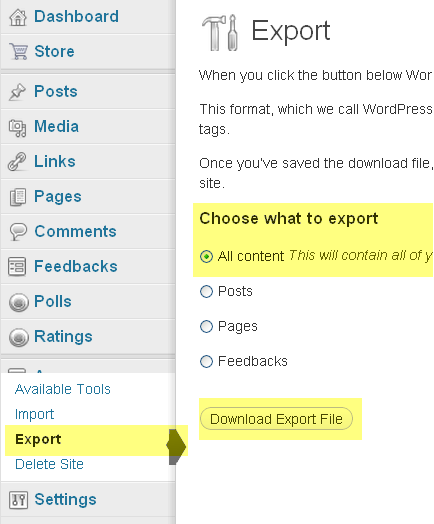
\includegraphics{toolsexport.png}}
%{[}/caption{]}
\captionsetup[figure]{labelformat=empty}
\begin{figure}[htbp]
\centering
\href{http://bakerjd99.files.wordpress.com/2012/02/toolsexport.png}{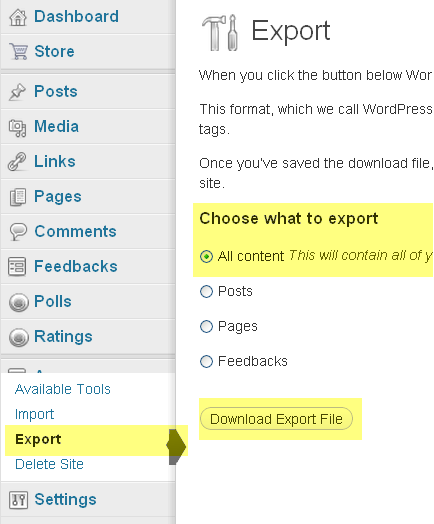
\includegraphics[width=0.23\textwidth]{toolsexport.png}}
\caption{Tools \textgreater{} Export \textgreater{} All  Content}
\label{fig:2518X1}
\end{figure}

When you press the \textbf{Download Export File} button your browser
will download a single XML file that contains all your posts and
comments. Remember where you save this file. I put my export XML here.
\begin{verbatim}
c:/pd/blog/wordpress/analyzethedatanotthedrivel.wordpress.xml
\end{verbatim}

\paragraph{Step 2: download \texttt{TeXfrWpxml.ijs}}

Download
\href{http://www.box.com/s/9v5b6ub9cya108c03mr7}{\texttt{TeXfrWpxml.ijs}}
and remember where you save it. I put this script here.
\begin{verbatim}
c:/pd/blog/TeXfrWpxml.ijs
\end{verbatim}

\paragraph{Step 3: start J and load \texttt{TeXfrWpxml.ijs}}

\texttt{TeXfrWpxml.ijs} was generated from
\href{http://bakerjd99.wordpress.com/the-jod-page/}{JOD dictionaries}.
With JOD it's easy to capture root word dependencies and produce
complete standalone scripts. \texttt{TeXfrWpxml.ijs} needs only the
standard J load profile to run. It does not require any libraries or
external references and should run on all Windows and Linux versions of
J after 6.02. Loading this script is a simple matter of executing:
\begin{verbatim}
load 'c:/pd/blog/TeXfrWpxml.ijs'
\end{verbatim}


The following shows this script running in a J 7.01 console. The console
is the most stripped down J runtime.
%\href{http://bakerjd99.files.wordpress.com/2012/02/wp2texjconsole.png}{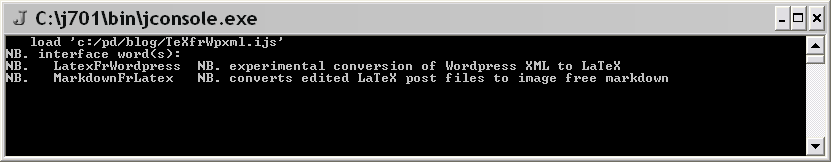
\includegraphics{wp2texjconsole.png}}
\begin{figure}[htbp]
\centering
\href{http://bakerjd99.files.wordpress.com/2012/02/wp2texjconsole.png}{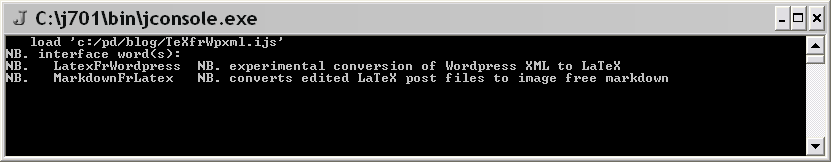
\includegraphics[width=\textwidth]{wp2texjconsole.png}}
\label{fig:2518X2}
\end{figure}

\paragraph{Step 4: review directories and necessary \LaTeX\ files}

The conversion script assumes proper directories are available up: see
\href{http://bakerjd99.wordpress.com/2012/02/18/wordpress-to-latex-with-pandoc-and-j-latex-directories-part-2-2/}{Part
2}. The first time you run \texttt{TeXfrWpxml.ijs} it's a good idea to
check that the directories and files the script is expecting are the
ones you want to process. You can verify the settings by displaying
\texttt{TEXFRWPDIR, TEXINCLUSIONS, TEXROOTFILE} and
\texttt{TEXPREAMBLE}.

%[sourcecode wraplines="false" gutter="false" autolinks="false"]
\begin{lstlisting}[language=jdoc,frame=single,framerule=0pt,label=lst:scr2518X0]
  TEXPREAMBLE
bmamble.tex
  TEXFRWPDIR
c:/pd/blog/wp2latex/
  TEXINCLUSIONS
inclusions
  TEXROOTFILE
bm.tex
  TEXPREAMBLE
bmamble.tex
\end{lstlisting}

If all these directories and files exist go to step (5).

\paragraph{Step 5: make sure you are online}

The first time you run the converter it will attempt to download all the
images referenced in your blog. This is where \texttt{wget.exe} gets
executed. Obviously to download anything you must be connected to the
Internet.

\paragraph{Step 6: run \texttt{LatexFrWordpress}}

Run the verb \texttt{LatexFrWordpress}. The monadic version of this verb
takes a single argument: the complete path and file name of the export
XML file you downloaded in step (1).

\footnotesize
\begin{verbatim}
xml=: 'c:/pd/blog/wordpress/analyzethedatanotthedrivel.wordpress.xml'

LatexFrWordpress xml
\end{verbatim}
\normalsize

As the verb runs you will see output like:


%[sourcecode wraplines="false" gutter="false" autolinks="false"]
% use empty language= lstlisting -- unbalanced ' chars in text
\begin{lstlisting}[language=,frame=single,framerule=0pt,label=lst:scr2518X1]
   LatexFrWordpress xml
What's In it for Facebook?
downloading: c:/pd/blog/wp2latex/inclusions/demotivational-posters-facebook-you.jpg
1 downloaded; 0 not downloaded; 0 skipped
Fake Programming
downloading: c:/pd/blog/wp2latex/inclusions/672169130_vajvn-M.png
1 downloaded; 0 not downloaded; 0 skipped
Laws or Suggestions
downloading: c:/pd/blog/wp2latex/inclusions/i-B5mfdRF-M.jpg
1 downloaded; 0 not downloaded; 0 skipped
Lens Lust

... many lines omitted ...

downloading: c:/pd/blog/wp2latex/inclusions/i-mNK4RHL-M.png
1 downloaded; 0 not downloaded; 0 skipped
WordPress to LaTeX with Pandoc and J: LaTeX Directories (Part 2)
0 downloaded; 0 not downloaded; 1 skipped
+-++
|1||
+-++
\end{lstlisting}

When the verb terminates you should have a directory
\texttt{c:/pd/blog/wp2latex} full of \texttt{*.tex} files: one file for
each blog post. Now the hard work starts.

\paragraph{Step 7: editing \LaTeX\ posts}

The conversion from WordPress XML to \LaTeX\ produces files that require
manual edits. The more images, video, tables and other elements in your
posts the more demanding these edits will become. My blog has about one
image per post. Most of these images are wrapped by text. \LaTeX\ has a
mind of its own when it comes to \emph{floating figures} and getting
illustrations to behave requires far more parameter tweaking than it
should. This is a longstanding weakness of \LaTeX\ that pretty much
everyone bitches about. My advice is start at the front of your document
and work through it post by post. The files generated by
\texttt{LatexFrWordpress} do not attempt to place figures for you but
they do bolt in ready-made figure templates as comments that you can
experiment with. Each post file is also set up for separate \LaTeX\
compilation. You don't have to compile your entire blog to tweak one
post. The one good thing about this edit step is once you have sorted
out your old posts you do not have to revisit them unless you make major
global document changes. The next time you run \texttt{LatexFrWordpress}
it will only bring down new posts and images.

\paragraph{Step 8: compile your \LaTeX\ blog}

I use batch files and shell scripts to drive \LaTeX\ compilations. I
processed my blog with this batch file.

%[sourcecode wraplines="false" gutter="false" autolinks="false"]
\begin{lstlisting}[language=bat,frame=single,framerule=0pt,label=lst:scr2518X2]
echo off
rem process blog posting (bm.tex) root file
title Running Blog Master/LaTeX ...

rem first pass for aux file needed by bibtex
lualatex bm

rem generate/reset bbl file
bibtex bm
makeindex bm

rem resolve all internal references - may
rem comment out when debugging entire document
lualatex bm
lualatex bm

rem display pdf - point to prefered PDF reader
title Blog Master/LaTeX complete displaying PDF ...
"C:\Program Files\SumatraPDF\SumatraPDF.exe" bm.pdf
\end{lstlisting}

The presence of Unicode APL, see
\href{http://bakerjd99.wordpress.com/2010/11/12/the-return-of-apl-fingers-2/}{this
post}, forced me to use lua\LaTeX. I needed some very
nonstandard APL fonts. \textbf{See
\href{http://www.box.com/s/8yvm27ag9agtm32nfahd}{bm.pdf} --- also
available on the \href{http://bakerjd99.wordpress.com/download-this-blog/}{\emph{Download this Blog}} page ---} to judge the
effectiveness of my edits. Producing nice figure laden typeset blog
documents is work but, as I will describe in the next post,
\emph{producing image free eBooks is a simple and far less laborious
variation on this process}.

%\captionsetup[floatingfigure]{labelformat=empty}
%\begin{figure}[htbp]
%\begin{floatingfigure}[l]{0.25\textwidth}
%\centering
%
\includegraphics[width=0.23\textwidth]{i-mNK4RHL-M.png}
%\caption{~~~IMCAPTION~~~}
%\label{fig:2518X0}
%\end{floatingfigure}
%\end{figure}

%\captionsetup[floatingfigure]{labelformat=empty}
%\begin{figure}[htbp]
%\begin{floatingfigure}[l]{0.25\textwidth}
%\centering
%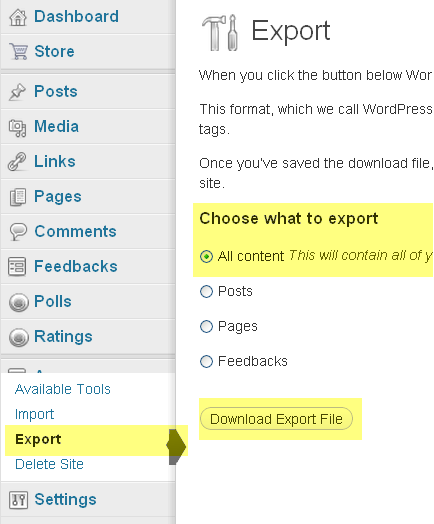
\includegraphics[width=0.23\textwidth]{toolsexport.png}
%\caption{~~~IMCAPTION~~~}
%\label{fig:2518X1}
%\end{floatingfigure}
%\end{figure}

%\captionsetup[floatingfigure]{labelformat=empty}
%\begin{figure}[htbp]
%\begin{floatingfigure}[l]{0.25\textwidth}
%\centering
%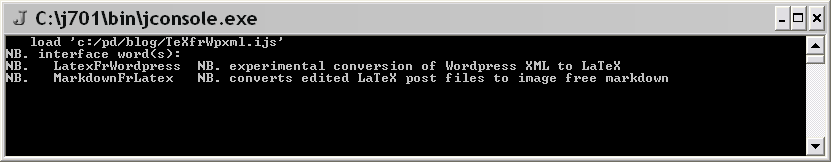
\includegraphics[width=0.23\textwidth]{wp2texjconsole.png}
%\caption{~~~IMCAPTION~~~}
%\label{fig:2518X2}
%\end{floatingfigure}
%\end{figure}


%\end{document}